\newcommand{\putrow}[3]{
\path (0,#1) node{#2} ++(0:1) node{#3};
}

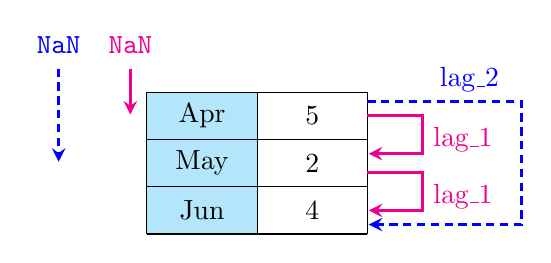
\begin{tikzpicture}[xscale=1.4,yscale=.6]
\begin{scope}[shift={(-.5,.5)}]
\fill[cyan!30] (0,0) rectangle +(1,-3);
\draw (0,0) grid (2,-3);
\end{scope}

\begin{scope}[-stealth,magenta,shorten >=.5pt,
every node/.style={midway,scale=1}]
\draw[line width=0.4mm] (1.5,0)--(2,0)--(2,-0.8)--(1.5, -0.8)    node[right, xshift=10, yshift=5]{lag\_1};
\draw[line width=0.4mm] (1.5,-1.2)--(2,-1.2)--(2,-2)--(1.5, -2)    node[right, xshift=10, yshift=5]{lag\_1};

\draw[line width=0.4mm] (-0.65, 1)--(-0.65, 0)    node[above, yshift=10]{\texttt{NaN}};
\end{scope}

\begin{scope}[-stealth,blue,shorten >=.5pt,
every node/.style={midway,scale=1}]
\draw[line width=0.4mm][densely dashed] (1.5,0.3)--(2.9,0.3)--(2.9,-2.3)--(1.5, -2.3)    node[above, xshift=9, yshift=44]{lag\_2};

\draw[line width=0.4mm][densely dashed] (-1.3, 1)--(-1.3, -1)    node[above, yshift=18.5]{\texttt{NaN}};

\end{scope}

\putrow{0}{Apr}{5}
\putrow{-1}{May}{2}
\putrow{-2}{Jun}{4}
\end{tikzpicture}
